\section{The Method of Green's Functions}
\setcounter{example}{0}
\subsection{Introduction}
A \df{Green's function} is the solution to a differential equation of the form
\begin{equation} \label{eq:greensdef}
    \opp{L^*_\xi} G(\xi, x) = \delta(\xi - x). 
\end{equation}
The subscript \(\xi\) on the differential operator indicates that the derivatives are being taken with respect to the variable \(\xi\). By making use of some of the delta function's unusual properties, Green's functions can be used to solve nonhomogeneous linear differential equations.

To find the solution to the linear differential equation
\begin{equation} \label{eq:4.2}
    \opp{L}u=\phi,
\end{equation}
we start by finding the formal adjoint as in equation (\ref{eq:adjoint}). If we replace \(v\) with \(G\), and we replace \(x\) with a dummy variable \(\xi\), we are left with an equation of the form
\begin{equation} \label{eq:greenadjoint}
    \intl G(\xi, x)\opp{L}u(\xi) d\xi = \bterms + \intl u(\xi)\opp{L^*}G(\xi,x) d\xi.
\end{equation} 
It follows from equation (\ref{eq:greensdef}) that we can replace \(\opp{L^*}G\) with \(\d\), and from equation (\ref{eq:4.2}) that we can replace \(\opp{L}u\) with \(\phi\), 
\begin{equation}
    \begin{split}
        \intl G(\xi,x)\phi(\xi) d\xi &= \bterms + \intl u(\xi)\d(\xi-x) d\xi\\
        &=\bterms + u(x).
    \end{split}
\end{equation}
Therefore, if we choose boundary conditions for \(G\) such that the boundary terms do not depend on \(u\) and we are able to find \(G\), then finding \(u\) is reduced to a problem of integrating \(G\phi\). 

To illustrate the key ideas of the method, we will consider several examples which begin simply and become more complex. Each example will be concerned with a key concept in implementing the method of Green's functions.
\subsection{Examples}
\begin{example} %add to table to contents
    \textit{Loaded String}
    
    Consider the boundary value problem
    \begin{equation} \label{ex1:initialize}
        u''(x) = \phi(x);\quad u(0)=u(1)=0
    \end{equation}
    where \(\phi(x)\) is prescribed. Equation (\ref{ex1:initialize}) can be regarded as describing the static deflection of a string under unit tension between fixed endpoints and subjected to a force distribution \(\phi(x)\).

    \begin{figure}\label{fig:LoadedString}
    \centering
    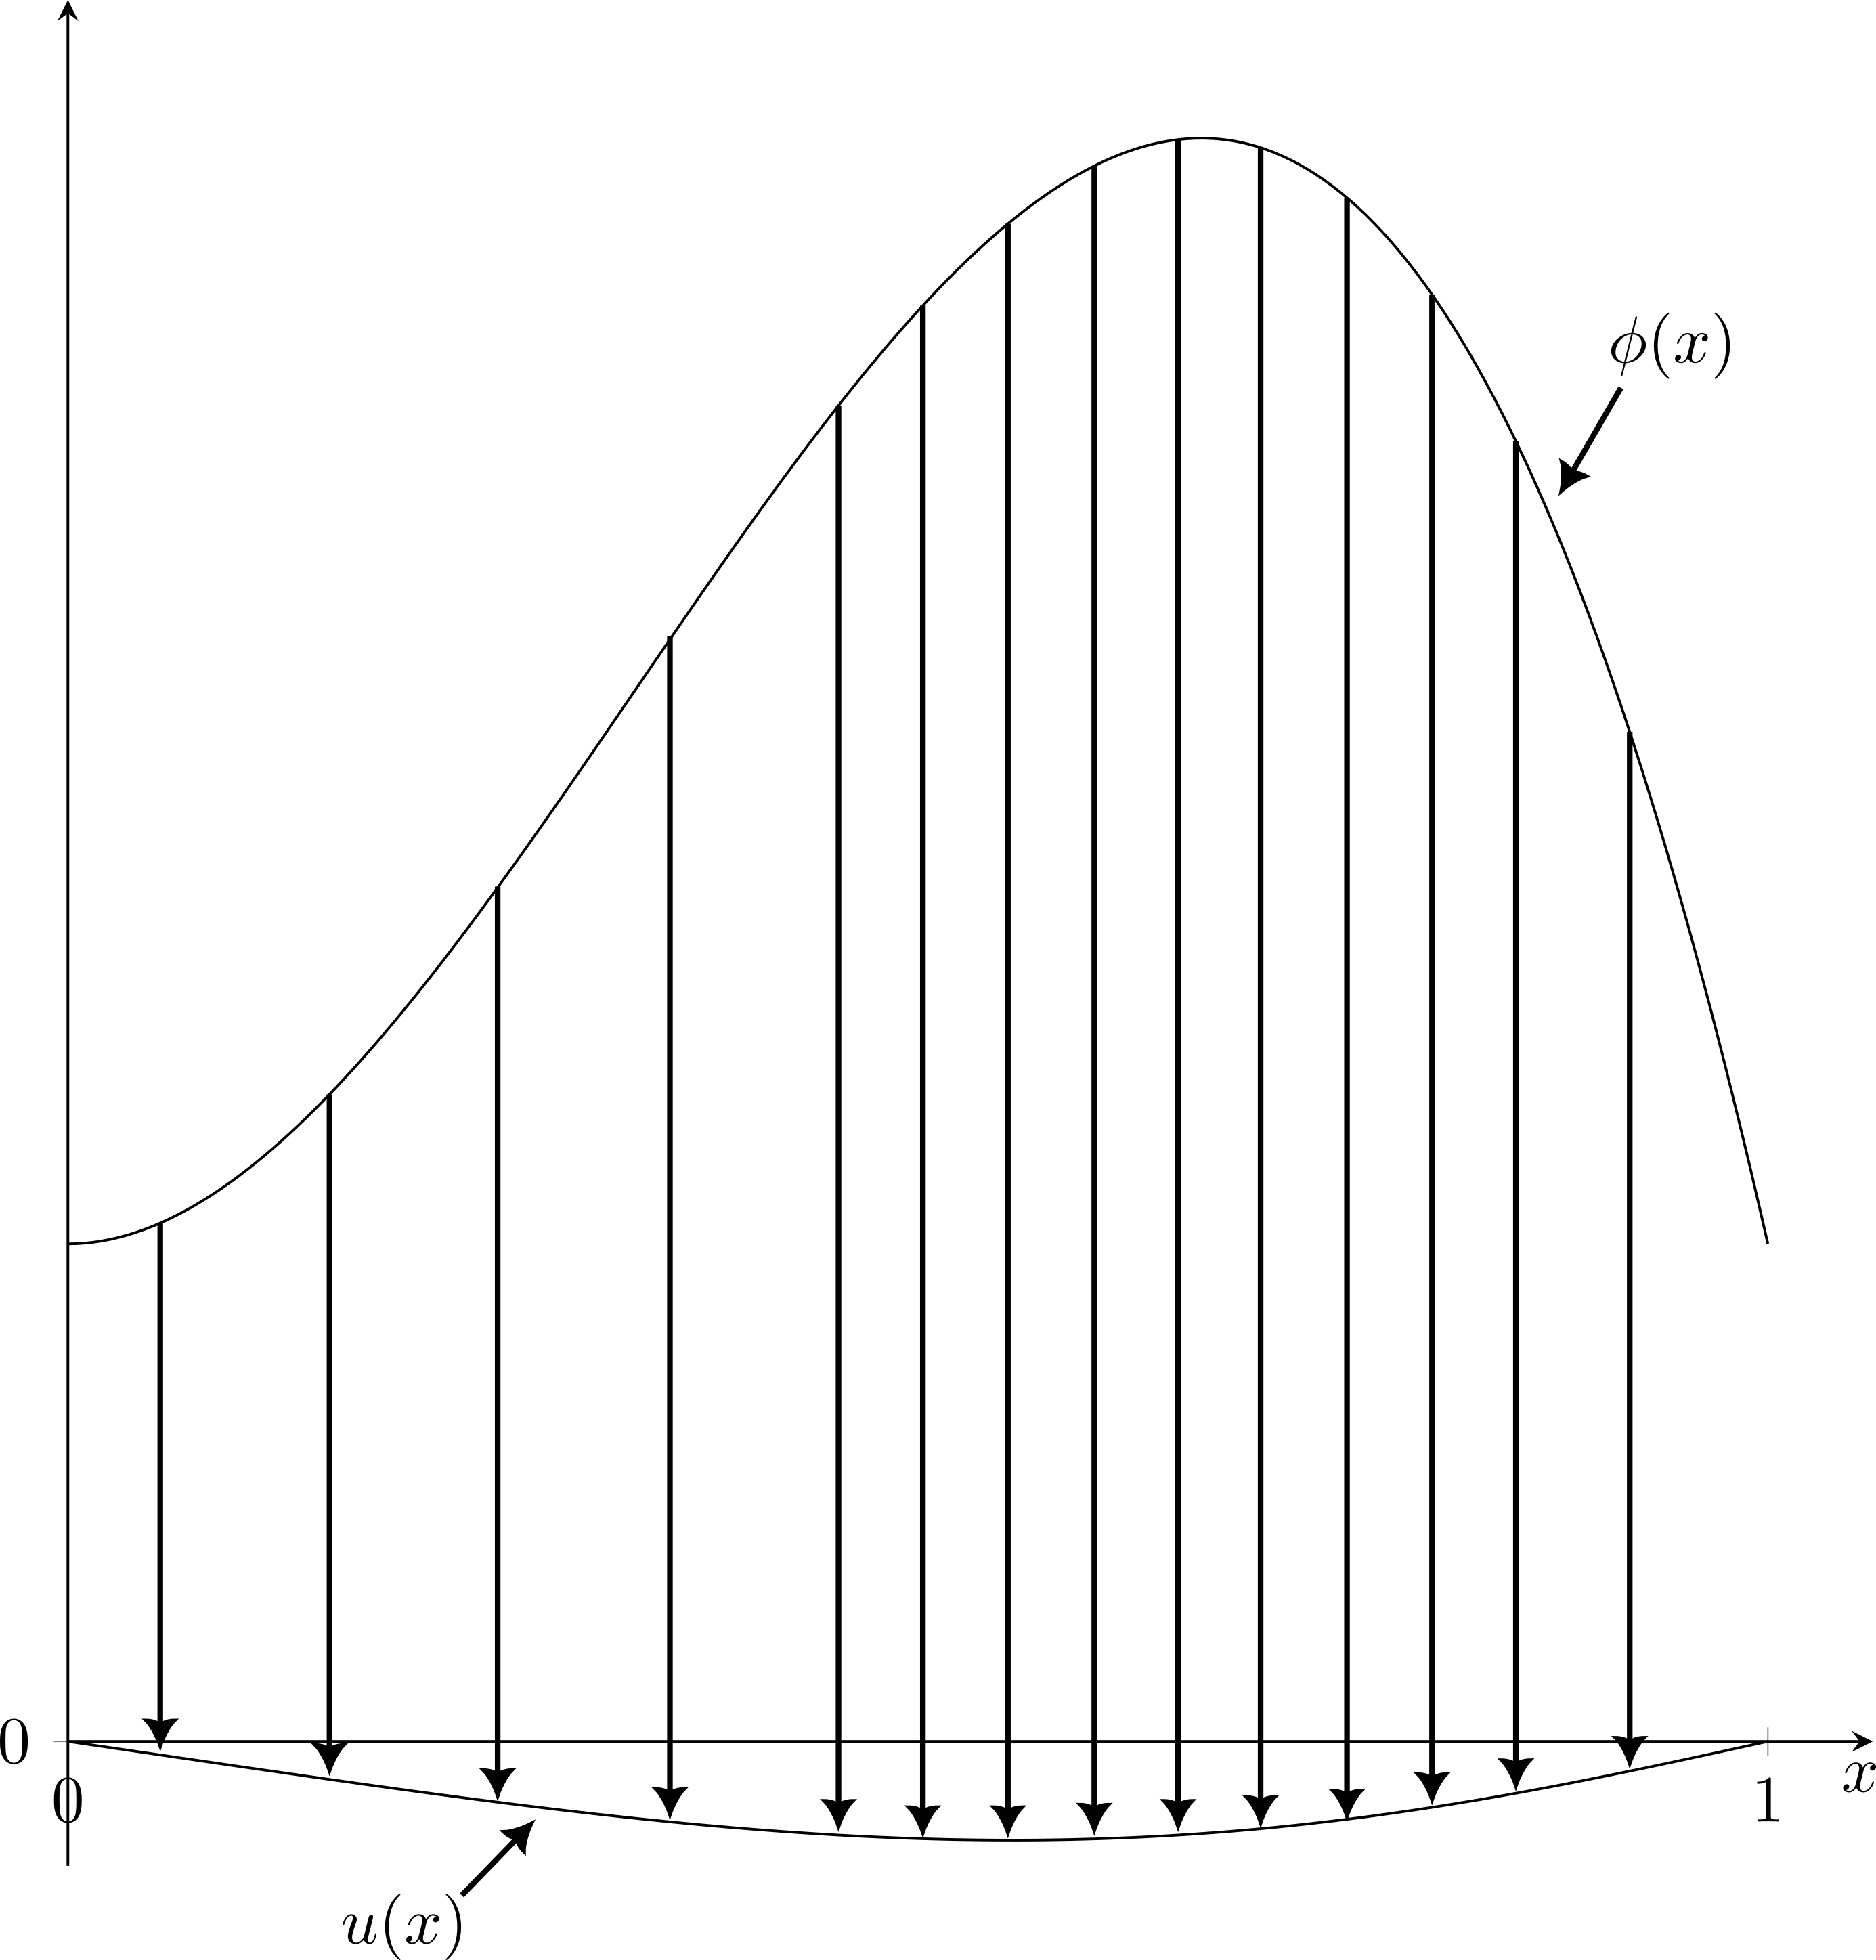
\includegraphics[width=0.5\linewidth]{include/loadedstring.png}
    \caption{Loaded String}
\end{figure}
    
    To find a solution to this differential equation, we first find the formal adjoint \(\L*\) as in equation (\ref{eq:greenadjoint}). 
    \begin{equation}
        \begin{split}
            \int_{0}^{1} G(\xi, x)\L u(\xi) d\xi  &= (G(\xi, x)u'(\xi)-G_\xi (\xi, x)u(\xi))\biggr\rvert_0^1 + \int_{0}^{1} uG_{\xi\xi}d\xi\\
            &= G(1, x)u'(1) - G_\xi(1, x)u(1) \\&- G(0, x)u'(0) + G_\xi(0,x)u(0) + \int_{0}^{1} uG_{\xi\xi}d\xi.
        \end{split}
    \end{equation}
    Therefore, 
    \begin{equation}
        \Lstar = \frac{d^2}{d\xi^2}
    \end{equation}
    and 
    \begin{equation}\label{eq:loadedStringLstarG}
        \Lstar G = G_{\xi\xi} = \delta(\xi-x).
    \end{equation}
    Because of the boundary conditions on \(u\) in equation (\ref{ex1:initialize}), two of our boundary terms are zero. Thus,
    \begin{equation}
        \int_{0}^{1} G(\xi, x)\L u(\xi) d\xi = G(1, x)u'(1) - G(0, x)u'(0) + \int_{0}^{1} uG_{\xi\xi}d\xi.
    \end{equation}
    Now, we want to remove the \(u\) dependency from the boundary terms and, as such, decide that
    \begin{equation}
        G(1,x) = G(0,x) = 0.
    \end{equation}
    Then the solution is given by 
    \begin{equation}\label{eq:loadSln}
        u(x) = \int_0^1 G(\xi,x)\phi(\xi)d\xi.
    \end{equation}
    To calculate the Green's function, we integrate equation (\ref{eq:loadedStringLstarG}), regarding \(x\) as fixed.
    \begin{equation}
        \begin{split}
            G_\xi &= H(\xi-x) + A\\
            G &= (\xi - x)H(\xi-x)+A\xi +B
        \end{split}
    \end{equation}
    Imposing the boundary conditions, 
    \begin{equation}
        \begin{split}
            &G(0,x) = 0 = B\\
            &G(1,x) = 0 =  1 - x + A + B,
        \end{split}
    \end{equation}
    shows us that \(B=0\) and  \(A=x-1\). Therefore
    \begin{equation}
        G(\xi,x) = (\xi-x)H(\xi-x) + (x-1)\xi.
    \end{equation}

    Equation (\ref{eq:loadedStringLstarG}) can, like equation (\ref{ex1:initialize}), be interepreted as the deflection of a loaded string. Specifically it is the deflection as a function of \(\xi\) due to a point load of unit strength, \(\d(\xi-x)\), instead of a load distribution, \(\phi\). Rewriting our Green's function as
    \begin{equation}
        G(\xi,x)= \begin{cases}
            (x-1)\xi, & \xi \leq x\\
            (\xi-1)x, & \xi \geq x
        \end{cases}
    \end{equation}
    makes it clear that \(G(\xi,x)\) is symemtric, \(G(\xi,x)=G(x,\xi)\). This is often referred to as "Maxwell Reciprocity." Because 
\end{example}
